\section{Anforderungsspezifikation}
\label{sec:Anforderungsspezifikation}

\subsection{Use Cases}
\label{sub:Use Cases}
Im folgenden sind die funktionalen Anforderungen an PlazaRoute mit all seinen Komponenten, welche im Kapitel \ref{sec:Architektur} aufgeführt sind, als Use Cases im Brief-Format beschrieben. Zur Übersicht ist das Use Case Diagramm in Abbildung \ref{fig:usecase_diagram} zu betrachten.

\begin{figure}[ht]
\centering
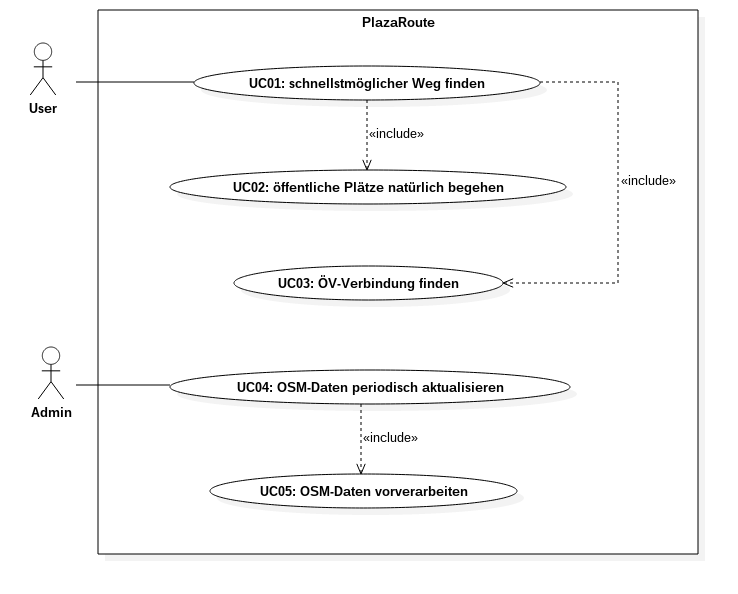
\includegraphics[width=1\linewidth]{projectdoc/img/usecase_diagram}
\caption[Use Case Diagramm]{Use Case Diagramm}
\label{fig:usecase_diagram}
\end{figure}

\subsubsection{Aktoren}
\label{useccase:Aktoren}

\begin{table}[h]
    \centering
    \caption{Aktoren}
    \label{aktoren}
    \begin{tabular}{ll}
        \textbf{Aktor} & \textbf{Beschreibung und Interessen}                                                                                                                                                                                     \\
        \textbf{User}  & \begin{tabular}[c]{@{}l@{}}Ein User ist ein Fussgänger, welcher schnellstmöglich von Punkt A zu Punkt B kommen möchte. \\ Er fungiert in der Komponente QGIS-Plugin.\end{tabular}                                          \\
        \textbf{Admin} & \begin{tabular}[c]{@{}l@{}}Ein Admin ist daran interessiert, dass aktuelle Daten dem Aktor User zur Verfügung stehen. \\ So möchte er Daten vorverarbeiten und dem Aktor User diese zur Verfügung stellen können.\end{tabular}
    \end{tabular}
\end{table}

\subsubsection{UC01: schnellstmöglicher Weg finden}
\label{usecase:UC01}
Aktoren: \emph{User}

Include: \nameref{usecase:UC02}, \nameref{usecase:UC03}

Nachdem der User einen Start- und Endpunkt (geografische Standorte) angegeben hat, erhält er den schnellstmöglichen Weg, welcher mit öffentlichen Verkehrsmitteln und zu Fuss machbar ist.

\subsubsection{UC02: Flächen im urbanen Raum natürlich begehen}
\label{usecase:UC02}
Aktoren: \emph{User}

Der User wird beim Fussgänger-Routing über Flächen im urbanen Raum auf direktem Weg natürlich (Definition im Kapitel \ref{criteria:Natürlichkeit} im Teil \ref{chap:Technischer Bericht}) geroutet. Dies betrifft insbesondere das Umgehen von Hindernissen.

\subsubsection{UC03: ÖV-Verbindung finden}
\label{usecase:UC03}
Aktoren: \emph{User}

Der User wird zu Fuss zu einer ÖV-Haltestelle geroutet, welche sich in einem Umkreis von 1 km befindet. Falls mehrere ÖV-Haltestellen verfügbar sind, wird die ÖV-Haltestelle gewählt, welche die kürzeste Reisezeit (Fussweg + ÖV-Weg) hat.

\subsubsection{UC04: OSM-Daten periodisch aktualisieren}
\label{usecase:UC04}
Aktoren: \emph{Admin}

Include: \nameref{usecase:UC05}

Der Admin aktualisiert die \ac{OSM}-Daten, auf welche in \nameref{usecase:UC01} geroutet wird, periodisch und integriert sie in die Routing-Engine.

\subsubsection{UC05: OSM-Daten vorverarbeiten}
\label{usecase:UC05}
Aktoren: \emph{Admin}

Der Admin führt die Vorverarbeitung der \ac{OSM}-Daten durch. Unter Vorverarbeitung versteht man das Einzeichnen von Fusswegen auf Flächen im urbanen Raum. Diese Daten werden der Routing-Engine übergeben und ermöglicht, dass die Routing-Engine den schnellstmöglichen Weg über Flächen im urbanen Raum finden kann.

\subsection{Nicht-funktionale Anforderungen}
\label{sub:Nicht-funktionale Anforderungen}

\subsubsection{NFA01: Docker-Images}
\label{NFA:NFA01}

PlazaRoute wird in Docker-Images ausgeliefert, um eine Verfügbarkeit auf unterschiedlichen Systemen sicherstellen und um das Deployment vereinfachen zu können.

\subsubsection{NFA02: austauschbare Routing-Engine}
\label{NFA:NFA02}

Die Routing-Engine, welche von PlazaRoute verwendet wird, soll austauschbar sein. Dabei soll nur die konkrete Implementation des Services, welche fürs Routing genutzt wird, angepasst werden müssen.

\subsubsection{NFA03: periodische Aktualisierung der OSM-Daten}
\label{NFA:NFA03}

Die \ac{OSM}-Daten werden wöchentlich für ein optimiertes Fussgänger-Routing über Flächen im urbanen Raum vorverarbeitet und der Routing-Engine übergeben.


\subsubsection{NFA04: Dauer der Vorverarbeitung}
\label{NFA:NFA04}

Die Vorverarbeitung der \ac{OSM}-Daten (Optimierung auf Flächen im urbanen Raum) darf maximal 2 Stunden dauern.

\subsubsection{NFA05: zusätzliche Datenmenge}
\label{NFA:NFA05}

Die zusätzlichen Daten für die Optimierung (zusätzlich eingezeichnete Wege über Flächen im urbanen Raum) dürfen nicht mehr als 1\% des Kartenmaterials betragen.

\subsubsection{NFA06: Dauer des Unterbruchs bei OSM-Daten-Integration}
\label{NFA:NFA06}

PlazaRoute ist während dem Integrieren der neuesten \ac{OSM}-Daten in die Routing-Engine maximal 2 Stunden nicht verfügbar. Der User wird nicht über den Unterbruch informiert.
